% Step-by-step delta-KB creation where the delta ADDS beyond canonical.
% Real data: Soybean / Cercospora Blight / Alabama / Bugwood 5581645
% (phase0r_traces.jsonl + Soybean registry + validate_kb Claude verifier).
\begin{figure*}[t]
\centering
\resizebox{\textwidth}{!}{%
\begin{tikzpicture}[
  font=\scriptsize,
  box/.style={draw, rounded corners=4pt, align=left, inner sep=6pt, text width=4.0cm, very thick},
  ttl/.style={font=\scriptsize\bfseries\sffamily},
  arr/.style={-{Stealth[length=3mm]}, very thick, black!55},
]
% (1) Canonical KB
\node[box, fill=green!5, draw=green!45] (c1) {
  {\bfseries\sffamily\color{green!45!black}\,1 $\cdot$ Canonical KB}\\[3pt]
  Cercospora Blight (Soybean)\\[2pt]
  \textit{``light purple spots\dots expand and deepen in color to a
  \textbf{reddish-purple or bronze}.''}\\[3pt]
  {\tiny\faGlobe~source: UMN Extension\\\url{https://extension.umn.edu/soybean-pest-management/cercospora-leaf-blight-and-purple-seed-stain-soybean}}
};
% (2) Swarm specialists
\node[box, right=0.8cm of c1, fill=purple!5, draw=purple!45] (c2) {
  {\bfseries\sffamily\color{purple!45!black}\,2 $\cdot$ Swarm --- specialists fire}\\[3pt]
  \begin{center}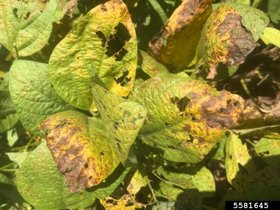
\includegraphics[width=1.35cm]{figures/delta_trace_cercospora.jpg}\end{center}
  {\tiny\faImage~Bugwood \#5581645 $\cdot$ Alabama (E.\ Sikora, Auburn)}\\[2pt]
  organ router $\to$ leaf group, 2 rounds:\\[1pt]
  $\circ$ \textit{LesionColor}: tan centre, chocolate-brown margin, chlorotic halo\\
  $\circ$ \textit{Concentric}: target spots, concentric rings\\
  $\circ$ \textit{LesionShape}: irregular
};
% (3) Delta KB adds
\node[box, right=0.8cm of c2, fill=orange!6, draw=orange!55] (c3) {
  {\bfseries\sffamily\color{orange!50!black}\,3 $\cdot$ Delta KB --- \emph{adds} to canonical}\\[3pt]
  \textit{``tan / chocolate-brown lesions with \textbf{concentric target rings}
  and a chlorotic halo.''}\\[3pt]
  {\bfseries STAGE / COLOR REFINEMENT}: morphology the canonical
  ``light purple'' did \emph{not} specify.\\[2pt]
  {\tiny\texttt{image\_quote}: ``target spots with alternating light and dark concentric rings are present.''}
};
% (4) Web verification
\node[box, right=0.8cm of c3, fill=red!4, draw=red!45] (c4) {
  {\bfseries\sffamily\color{red!50!black}\,4 $\cdot$ Web verification}\\[3pt]
  {\bfseries Claude verifier} (Step~3, \texttt{validate\_kb}) web-searches
  extension / peer-reviewed sources; fabricated cites forbidden.\\[2pt]
  verdict: \textbf{provisional} $\to$ flagged for human review.\\[2pt]
  {\tiny\faCheckCircle~\texttt{web\_support} \{url, quote\}: UMN Ext.\
  ``\dots deepen in color to a reddish-purple or bronze'' --- corroborates the
  darker coloration the delta adds.}
};
\draw[arr] (c1) -- (c2);
\draw[arr] (c2) -- (c3);
\draw[arr] (c3) -- (c4);
\end{tikzpicture}
}%
\caption{\textbf{Delta KB that \emph{adds} to canonical --- step by step.} A real
trace for \emph{Soybean / Cercospora Blight} on one geo-tagged Alabama
\bugwood{} photograph (\#5581645). \textbf{(1)} the cited canonical text only
says ``light purple\dots bronze''; \textbf{(2)} the organ router fires the leaf
specialists, which on the two-round blackboard report tan/chocolate-brown
centres, concentric target rings, and a chlorotic halo; \textbf{(3)} the
consolidated \emph{delta} therefore \emph{extends} canonical with morphology it
omitted (a stage/color refinement, not mere captioning); \textbf{(4)} the
\textsc{Claude} web verifier assigns a status and attaches a \texttt{web\_support}
\{url, quote\} citation, leaving the refinement \emph{provisional} for human
adjudication. Both canonical and delta thus carry their own verifiable source.}
\label{fig:delta-trace}
\end{figure*}
